\documentclass{article}
\usepackage[fleqn]{amsmath}
\usepackage{bm}
\usepackage{amssymb}
\usepackage{graphicx}
\graphicspath{ {./graphics/} }
\usepackage[title]{appendix}
\usepackage{gensymb}
\usepackage[table]{xcolor}
\usepackage{authblk}
\newcommand{\Rho}{\mathrm{P}}
\title{Adam SLAM - the last mile of camera calibration with 3DGS}
\author[1,2]{Matthieu GENDRIN}
\author[1]{Stéphane PATEUX}
\author[2]{Xiaoran JIANG}
\author[1]{Théo LADUNE}
\author[2]{Luce MORIN}
\affil[1]{Orange Innovation}
\affil[2]{INSA}
\setlength{\parindent}{0cm}

\date{\today}
% Hint: \title{what ever}, \author{who care} and \date{when ever} could stand 
% before or after the \begin{document} command 
% BUT the \maketitle command MUST come AFTER the \begin{document} command! 
\begin{document}

\maketitle

\section{Introduction}
3d gaussian splatting \cite{kerbl20233d} has been a major breakthrough in the domain of 3D novel view synthesis, reaching state of the art quality with an
efficient, realtime rendering performance. The research community has been florishing since, but the quality improvements are generally expressed in fractions of dB.
For instance, MCMC \cite{kheradmand20243d} improved the PSNR of between 0.4dB and 0.7dB depending on the dataset.

In such a context, the quality of the camera calibration is of major importance, each error of one pixel having an impact in the order of 
magnitude of a dB PSNR. The calibration is a field of research in itself, which not focusses on quality but seeks 
the best balance between precision, robustness and compute efficiency. The state of the art is held by feature based algorithms,
with COLMAP \cite{schonberger2018robust} as a reference, and many proposals to improve the tracks of features used in that algorithm.
Such solutions give a calibration suitable for novel view synthesis algorithms to converge. In some circumstances though, the calibration
introduces some errors, for example with low-textured scenes, or when features are very unevenly distributed throughout the scene. 
The hard point about evaluating the quality of calibration is that we don't have a ground truth for real scenes. At the end of the day,
the quality of the calibration is assessed by the quality of the novel view synthesis.

Taking this into consideration, some publications train the pose of the camera based on the loss of the novel view synthesis itself, like 
gsplatloc \cite{zeller2024gsplatloc} which generates a depthmap from a 3dgs model and compares it with a ground truth, or gsplat \cite{ye2024gsplat}
which backpropagates on the pose of the camera during the 3dgs training. Similar to this last publication, we train a 3dgs model from
a pre-existing calibration, and fine-tune this calibration based on the color loss of the novel view synthesis. Unlike gsplat though,
we focus some iterations of the training on calibration improvement, use a L2 loss in these iterations which performs better than L1,
and train the focal length of the cameras on top of the pose. We also propose a reparameterization of the camera extrinsics and intrinsics
for a more efficient training. These changes improve the final quality of the calibration, reaching an average 0.4dB PSNR improvement
on the ref dataset of \cite{kerbl20233d}.

\section{Method} \label{method}

The main idea of this paper is basically to use backpropagation to train camera parameters from the color loss, we
will develop some more details about the appropriate way to perform this training. 
Section \ref{backprop} explain how backpropagation can be simplified for implementation ease.
The choise of the color loss is discussed in section \ref{L2}.
Then the training schedule between model and camera fine-tuning is the subject of \ref{schedule}.
Finally, section \ref{abc} proposes a reparameterization of the camera model, for a more performant training with Adam optimizer.

\subsection{Backpropagation} \label{backprop}
The whole rendering is kept as is, except that the camera parameters are trained, based on the color loss.
Noting $p_j$ one parameter of camera $j$, the derivatives of the color loss $\mathcal{L}$ wrt $p$ are:
\begin{align}
	\label{eq:1}
	\frac{\partial \mathcal{L}}{\partial p_j} &= \sum_{i} \frac{\partial \mathcal{L}}{\partial uv_i} \frac{\partial uv_i}{\partial p_j} + \frac{\partial \mathcal{L}}{\partial cov2d_i} \frac{\partial cov2d_i}{\partial p_j}
\end{align}
With $uv_i$ the coordinates of the center and $cov2d_i$ the projection of the covariance matrix of the gaussian $i$ on image plan of the camera $j$.

We neglect the impact of $p_j$ on $cov2d_i$ in \eqref{eq:1}, leading to:
\begin{align}
	\label{eq:2}
	\frac{\partial \mathcal{L}}{\partial p_j} &= \sum_{i} \frac{\partial \mathcal{L}}{\partial uv_i} \frac{\partial uv_i}{\partial p_j}
\end{align}

This approximation is valid if $Cov_i << z_i$, which is the case for most gaussians in the model. Note that this approximation is
already done by \cite{kerbl20233d} when they approximate pinhole projection of the gaussian by an orthogonal projection.
In practice, we can notice that Colmap lack of precision usually happens on the z position versus the focal. Changing these parameters will have no impact on 
the transformation of the covariance from absolute referential to the relative referential, and small impact on the projection to the image plan.

\subsection{Choice of the loss} \label{L2}
While the choice of L1 loss has very good results in training gaussian model, we found that L2 (MSE) error is more
suitable to train the camera parameters. This can be interpreted as an effect of the lower importance of small
errors in L2 loss, thus making noise throughout the whole image negligeable before actual difference due to the 
calibration error.
Our experiments shows that L1 can lead the system to diverge, ending with trained cameras parameters worse than
the input ones.

This difference in loss implies to dedicate some iterations to camera parameters training. This split between
model training iterations and camera training iterations extends the total duration of training but enable
more precise and reliable results.

\subsection{Training schedule} \label{schedule}
The model training uses the cameras calibration as an input, and vice versa. Concurrent training of interdependent
parameters are common in machine learning, and gsplat \cite{ye2024gsplat} trains camera parameters and the model in parallel.
We propose a different schedule, by phase, with a prioritization scheme to allow more compute time on cameras that need it.
We proceed in a loop with M iterations of model training, followed by the training of the camera parameters, one camera
after another. One camera is trained for maximum 1000 steps, but a progress score is evaluated so that the training of the
camera is interrupted when the progress score reaches a minimum threshold t.

The progress score is an exponential moving average of the PSNR progress:
\begin{align}
	score_{n+1} &= score_n * (1 - \beta) + \beta (psnr_{n+1} - psnr_n) 
\end{align}
In our experiments, we use $\beta = 0.02, M = 3000, t = 0.0002$.

This enables us to save training iterations on cameras whose training does not improve the PSNR. In our 
experiments, this leads to 20\% savings in cameras training.

\subsection{Reparameterization} \label{abc}
Consider the pinhole projection of the center of one gaussian whose position to the camera is $x,y,z$:
\begin{align}
	\label{eq:uv}
	(u, v) &= (\frac{f_x}{z} x, \frac{f_y}{z} y)
\end{align}
We can see from \ref{eq:uv} that any modification of the camera parameters that keeps $(f_x / z, f_y / z)$ constant will have no
impact of $(u,v)$. In a degenerate scene with all gaussians at the same $z$, it would not be possible to desentangle the parameters.
Fortunately, the distribution is such that this case never happens, but $f_x, f_y$ and $z$ are still highly correlated.
This correlation is related to the similarity between getting closer to the scene and zooming in with the camera. Note that in
3dgs \cite{kerbl20233d}, the focal $f_x, f_y$ parameters are replaced by the field of view, noted $\phi_x,\phi_y$.

To help training the model, the parameters $(z_c, \phi_x, \phi_y)$ of a camera can be replaced by others, $(a, b, c)$.
One reparameterization is to chose $(a, b, c)$ as the coordinates in the referential defined by the eigen vectors of the hessian matrix of $\mathcal{L}(z_c,\phi_x,\phi_y)$.
Calling $\mathcal{E}$ this matrix, we have simply:
\begin{align}
	\label{eq:abc}
	\begin{bmatrix}z_c\\\phi_x\\\phi_y\end{bmatrix} = \begin{bmatrix}z_{c}^0\\\phi_x^0\\\phi_y^0\end{bmatrix} + \begin{bmatrix}\mathcal{E}\end{bmatrix} \begin{bmatrix}a\\b\\c\end{bmatrix} \\
\end{align}
With highly correlated parameters, the eigen values of the hessian matrix are of very different values, which leads to parameters
$(a,b,c)$ having an impact of different orders of magnitude on the loss. Explicitely giving the disentangled parameters to the Adam optimizer
will enable it to better optimizer gradient descent.

Indeed, since Adam normalizes the gradient by the average norm of the precedent gradients, a reparameterization is not neutral.
Giving new parameters to Adam, the step applied by the optimizer to $a$ will be more or less the same as 
the step applied to $b$ or $c$, even though its gradient is smaller.

In practice, the first optim phase is done with the standard $(z_c,\phi_x,\phi_y)$ parameters, then the values of $(z_{c}^0,\phi_x^0,\phi_y^0)$ are set,
the hessian is evaluated, $(a,b,c)$ are initiated at $(0,0,0)$ and the rest of the optimization process is done with the same $(a,b,c)$ parameters.

Since the second derivation of the loss gives unstable results, we approximate the hessian by finite difference, evalated from the gradient on the current
$(z_c,\phi_x,\phi_y)$ and on points around it $(z_c \pm \epsilon, \phi_x \pm \epsilon, \phi_y \pm \epsilon)$.

\section{Results}

Our results are processed in two steps: we first train the camera positions and model together, as described in \ref{method},
then we re-train the model, render the test images and process metrics with the original code of \cite{kerbl20233d}.
The results are listed in table \ref{table:results}.

\begin{table}[h!]
	\begin{center}
		{\rowcolors{2}{white}{lightgray}
		\begin{tabular}{|p{3cm}|c|c|}
			\hline
			scene & dataset calib & ours \\
			\hline
			mip360 bicycle & 25.61 & \textbf{26.34} \\
			mip360 bonsai & 32.32 & \textbf{32.72} \\
				mip360 counter & 29.11 & \textbf{29.26} \\
				mip360 garden & 27.77 & \textbf{28.32} \\
				mip360 kitchen & \textbf{31.55} & 31.14 \\
				mip360 room & 31.72 & \textbf{31.94} \\
				mip360 stump & 26.90 & \textbf{27.28} \\
				T\&T Train & 22.12 & \textbf{22.61} \\
				T\&T Truck & 25.84 & \textbf{26.18} \\
				DB DrJohnson & 29.11 & \textbf{30.12} \\
				DB Playroom & 29.96 & \textbf{30.77} \\
				\hline
			\end{tabular}
			}
			\caption{PSNR on the ref scenes as defined by \cite{kerbl20233d}.
					 Column "dataset calibration" lists results of training using the Colmap calibration provided with the datasets.
					 Colum "ours" lists results of training with the exact same code but using calibration fine-tuned by our algorithm.}
			\label{table:results}
		\end{center}
\end{table}

One some images, one can see the slight calibration error of the Colmap input, and the result of the fine-tuning.
The Figure \ref{img:quali} shows a slight misalignment on Colmap \cite{schonberger2018robust}, visible on the wheel
of the bicycle, which is corrected by camera fine-tuning.

\begin{figure}
	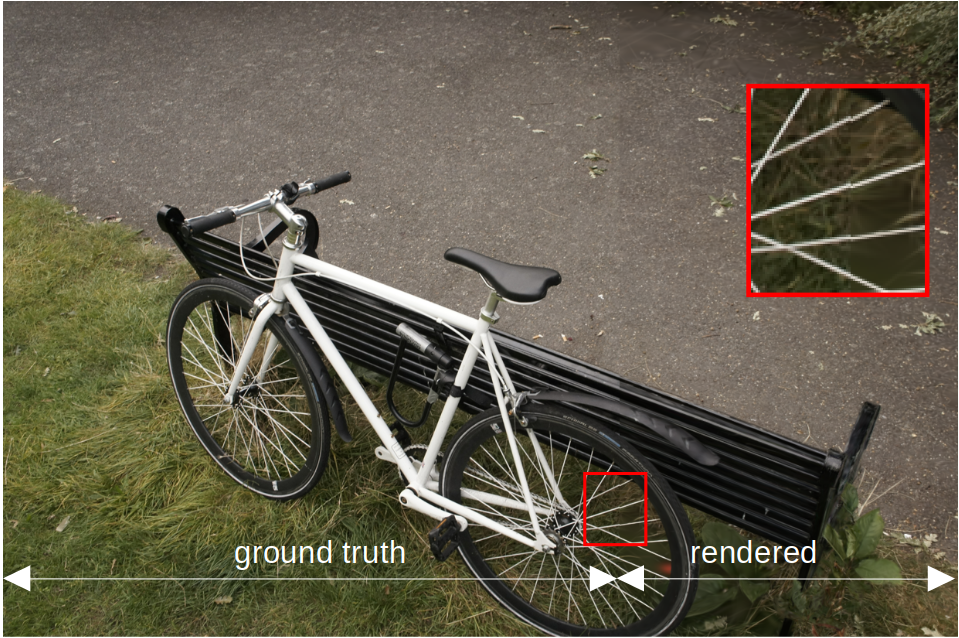
\includegraphics[width=6cm]{bicycle-ref2}
	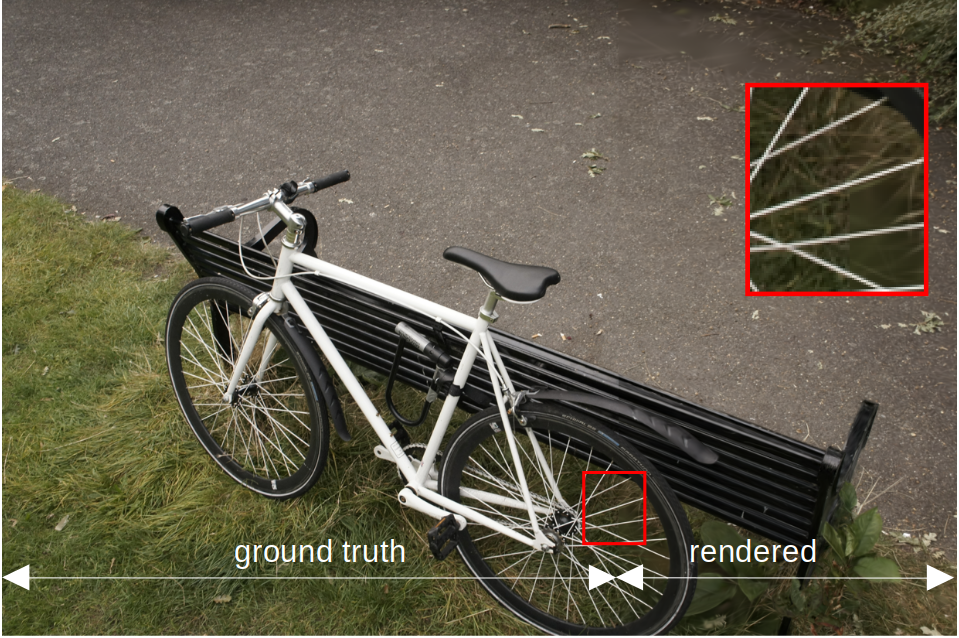
\includegraphics[width=6cm]{bicycle-calib2}
	\caption{Reference (left) vs ours (right)}
	\label{img:quali}
\end{figure}

\section{Conclusion}

Considering the precision of camera calibration as a matter of importance for the comparison of publications of
novel view synthesis, we propose a solution to fine tune this calibration. The camera calibration uses a 
3dgs model which is trained in parallel in an interleaved training schedule.
The new calibration alone brings an average improvement of 0.4dB PSNR on the dataset used as ref by 3dgs \cite{kerbl20233d}.
The fine tuning may be long and its suitability depends on the criticity of training time, but for calibration
of reference scenes, such as \cite{barron2022mip}, the stake of novel view quality is the most important.


\bibliographystyle{plain}
\bibliography{calibration}

\begin{appendices}
    
\section{Ablations}

\subsection{Fov training}

The table below gives the PSNR obtained by the same process as ours, but with one of the aspects missing.
The impact on PSNR is listed in the table \ref{table:ablation}.
\begin{itemize}
	\item w/o abc does not use reparameterization. Note that this is generally less performant, but not always.
	\item w/o fov does not train ($\phi_x, \phi_y$). Note that this implies not to use reparameterization neither.
	\item L1 uses L1 loss instead of L2, for camera parameters training.
\end{itemize}

\begin{table}[h]
	\begin{center}
	{\rowcolors{2}{white}{lightgray}
	\begin{tabular}{|p{3cm}|c|c|c|c|}
				\hline
				scene & w/o abc & w/o fov & L1 & full \\
				\hline
				mip360 bicycle & 25.81 & 25.74 & 25.82 & 26.34 \\
				mip360 bonsai & 32.31 & 32.15 & 32.41 & 32.72 \\
				mip360 counter & 29.04 & 29.09 & 29.13 & 29.26 \\
				mip360 garden & 27.70 & 27.50 & 27.72 & 28.32 \\
				mip360 kitchen & 31.12 & 31.07 & 30.71 & 31.14 \\
				mip360 room & 31.75 & 31.77 & 31.80 & 31.94 \\
				mip360 stump & 26.72 & 26.60 & 26.73 & 27.28 \\
				T\&T Train & 22.47 & 22.31 & 22.54 & 22.61 \\
				T\&T Truck & 26.13 & 26.05 & 26.11 & 26.18 \\
				DB DrJohnson & 29.93 & 29.55 & 29.81 & 30.12 \\
				DB Playroom & 31.61 & 30.36 & 30.45 & 30.77 \\
				\hline
			\end{tabular}
	}
	\caption{PSNR with and without fov training.}
	\label{table:ablation}
	\end{center}
\end{table}

\end{appendices}


\end{document}
